\documentclass[a4paper,12pt,twoside]{../includes/ThesisStyle}
\usepackage[utf8]{inputenc}
\usepackage[T1]{fontenc}

\usepackage[left=1.5in,right=1.3in,top=1.1in,bottom=1.1in,includefoot,includehead,headheight=13.6pt]{geometry}\renewcommand{\baselinestretch}{1.05}


% =============================================================================
%\usepackage[sectionbib]{chapterbib}	% Cross-reference package (Natural BiB)
%\usepackage{bibunits}
%\usepackage{natbib}					% Put References at the end of each chapter
\usepackage{algorithm}
\usepackage{alltt}
\usepackage{amsfonts}
\usepackage{amsmath}
\usepackage{amssymb}
\usepackage{cite}
\usepackage{color}
\usepackage{enumerate}
\usepackage{booktabs} % used for \midrule
\usepackage{fancyhdr}					% Fancy Header and Footer
\usepackage{graphicx}
\usepackage{ifthen}
\usepackage{latexsym}
\usepackage{multirow}
\usepackage{rotating}					% Sideways of figures & tables
\usepackage{stmaryrd}
\usepackage{subfigure}
\usepackage{url}         
\usepackage{xspace}
\usepackage[normalem]{ulem} % for \sout
\usepackage{xcolor}
\usepackage{tablefootnote}
\usepackage{pifont}

% =============================================================================

% Table of contents for each chapter
\usepackage[nottoc, notlof, notlot]{tocbibind}
\usepackage{minitoc}
\setcounter{minitocdepth}{1}
\mtcindent=15pt

\setcounter{secnumdepth}{3}
\setcounter{tocdepth}{2}
  
% =============================================================================
% Fancy Header Style Options

\pagestyle{fancy}                       % Sets fancy header and footer
\fancyfoot{}                            % Delete current footer settings

%\renewcommand{\chaptermark}[1]{         % Lower Case Chapter marker style
%  \markboth{\chaptername\ \thechapter.\ #1}}{}} %

%\renewcommand{\sectionmark}[1]{         % Lower case Section marker style
%  \markright{\thesection.\ #1}}         %

\fancyhead[LE,RO]{\bfseries\thepage}    % Page number (boldface) in left on even
% pages and right on odd pages
\fancyhead[RE]{\bfseries\nouppercase{\leftmark}}      % Chapter in the right on even pages
\fancyhead[LO]{\bfseries\nouppercase{\rightmark}}     % Section in the left on odd pages

\let\headruleORIG\headrule
\renewcommand{\headrule}{\color{black} \headruleORIG}
\renewcommand{\headrulewidth}{1.0pt}
\usepackage{colortbl}
\arrayrulecolor{black}

\fancypagestyle{plain}{
  \fancyhead{}
  \fancyfoot{}
  \renewcommand{\headrulewidth}{0pt}
}


% =============================================================================
% Clear Header Style on the Last Empty Odd pages
\makeatletter

\def\cleardoublepage{\clearpage\if@twoside \ifodd\c@page\else%
  \hbox{}%
  \thispagestyle{empty}%              % Empty header styles
  \newpage%
  \if@twocolumn\hbox{}\newpage\fi\fi\fi}

\makeatother

\newenvironment{maxime}[1]
{
\vspace*{0cm}
\hfill
\begin{minipage}{0.5\textwidth}%
%\rule[0.5ex]{\textwidth}{0.1mm}\\%
\hrulefill $\:$ {\bf #1}\\
%\vspace*{-0.25cm}
\it 
}%
{%

\hrulefill
\vspace*{0.5cm}%
\end{minipage}
}

\let\minitocORIG\minitoc
\renewcommand{\minitoc}{\minitocORIG \vspace{1.5em}}


\renewcommand{\epsilon}{\varepsilon}

% centered page environment
\newenvironment{vcenterpage}
	{\newpage\vspace*{\fill}\thispagestyle{empty}\renewcommand{\headrulewidth}{0pt}}
	{\vspace*{\fill}}
	

%=============================================================================

\usepackage{needspace}
\newcommand{\needlines}[1]{\Needspace{#1\baselineskip}}

\usepackage{xcolor}
\definecolor{source}{gray}{0.95}
% source code formatting
\usepackage{listings}
    % global settings for source code listing package
\lstset{
    basicstyle=\ttfamily\small,
    showspaces=false,
    showstringspaces=false,
    captionpos=b, 
    columns=fullflexible}

\lstdefinelanguage{ST}{
    keywordsprefix=\#,
    morekeywords=[0]{true,false,nil},
    morekeywords=[1]{self,super,thisContext},
    morekeywords=[2]{ifTrue:,ifFalse:,whileTrue:,whileFalse:,and:,or:,xor:,not:,by:,timesRepeat:},
    sensitive=true,
    morecomment=[s]{"}{"},
    morestring=[d]',
    escapechar={!},
    alsoletter={., :, -, =, +, <},
    moredelim=**[is][\itshape]{/+}{+/},
    literate=
        {^}{{$\uparrow$}}1
        {:=}{{$\leftarrow$}}1
        {~}{{$\sim$}}1
        {-}{{\sf -\hspace{-0.13em}-}}1  % the goal is to make - the same width as +
        {+}{\raisebox{0.08ex}{+}}1		% and to raise + off the baseline to match V
        , % Don't forget the comma at the end!
    style=STStyle
}
\lstdefinestyle{STStyle}{
    tabsize=4,
    %frame=leftline,
    % frame=bl,
    %framerule=2pt,
    %rulecolor=\color{gray},
    % backgroundcolor=\color{white},
    %backgroundcolor=\usebeamercolor[bg]{listing},
    basicstyle=\ttfamily\small,
    keywordstyle=\bf\ttfamily,
    % stringstyle=\color{orange},
    stringstyle=\mdseries\slshape,
    commentstyle=\it\rmfamily\color{darkgray}, 
    commentstyle=\mdseries\slshape\color{gray},
    %commentstyle=\mdseries\slshape,
    emphstyle=\bf\ttfamily,
    escapeinside={!}{!},
	%backgroundcolor=\color{source},
    %emphstyle={[2]\color{red}},
    %emphstyle={[3]\color{blue}\bf},
    %emphstyle={[4]\color{blue}},
    keepspaces=true
} 

%\lstnewenvironment{javacode}  [1][]{\lstset{language=java,#1}\needlines{#2}}{} 
%\lstnewenvironment{pythoncode}[2][]{\lstset{language=python,#1}\needlines{#2}}{}
\lstnewenvironment{stcode}    [2][]{\lstset{language=ST,#1}\needlines{#2}}{}
\lstnewenvironment{ccode}     [2][]
    {\lstset{language=C,numbers=left,escapechar=\$,numberstyle=\tiny,#1}\needlines{#2}}{}

% ON: I tried to pass the line number options in as arg #1 but it does not work for me
% I also could net get the line numbers to consistently increase
\lstnewenvironment{numstcode} [2][]
    {\lstset{language=ST,numbers=left,numberstyle=\tiny,numbersep=2pt,#1}\needlines{#2}}{}
\lstnewenvironment{numstcodecont} [2][]
    {\lstset{language=ST,numbers=left,numberstyle=\tiny,numbersep=2pt,firstnumber=last#1}\needlines{#2}}{}

\newcommand{\lst}[1]{{\tt #1}}

% In-line code (literal)

% In-line code (latex enabled)
% Use this only in special situations where \ct does not work
% (within Section headings ...):
\newcommand{\lct}[1]{{\textsf{\textup{#1}}}}
% Code environments
\lstnewenvironment{code}{%
	\lstset{%
		% frame=lines,
		frame=single,
		framerule=0pt,
		mathescape=false
	}
}{}

%\renewcommand{\lstlistingname}{Code Example}

% =============================================================================
\newboolean{showcomments}
\setboolean{showcomments}{true}

\ifthenelse{\boolean{showcomments}} {
	\newcommand{\ugh}[1] {\textcolor{red}{\uwave{#1}}}	% please rephrase
	\newcommand{\ins}[1] {\textcolor{blue}{\uline{#1}}}	% please insert
	\newcommand{\del}[1] {\textcolor{red}{\sout{#1}}}	% please delete
	\newcommand{\chg}[2] {								% please change
		\textcolor{red}{\sout{#1}}{\ra}
		\textcolor{blue}{\uline{#2}}}
	\newcommand{\nbc}[3]{								% comment
		{\colorbox{#3}{\bfseries\sffamily\scriptsize\textcolor{white}{#1}}}
		{\textcolor{#3}{\sf\small$\blacktriangleright$\textit{#2}$\blacktriangleleft$}}}

}{
	\newcommand{\ugh}[1]{#1}							% please rephrase
	\newcommand{\ins}[1]{#1}							% please insert
	\newcommand{\del}[1]{}								% please delete
	\newcommand{\chg}[2]{#2}							% please change
	\newcommand{\nbc}[3]{}								% comment
}

% =============================================================================
\usepackage[pagebackref,hyperindex=true]{hyperref}


% Links in pdf
\usepackage{color}
\definecolor{linkcol}{rgb}{0.0, 0.0, 0.0} 
\definecolor{citecol}{rgb}{0.0, 0.0, 0.0} 

% Change this to change the informations included in the pdf file
% See hyperref documentation for information on those parameters
\hypersetup {
	bookmarksopen=true,
	pdftitle="Design and Use of Anatomical Atlases for Radiotherapy",
	pdfauthor="Olivier COMMOWICK", 
	pdfsubject="Creation of atlases and atlas based segmentation", %subject of the document
	%pdftoolbar=false, % toolbar hidden
	pdfmenubar=true, %menubar shown
	pdfhighlight=/O, %effect of clicking on a link
	colorlinks=true,
	pdfpagemode=UseNone,
	pdfpagelayout=SinglePage,
	pdffitwindow=true,
	linkcolor=linkcol,
	citecolor=citecol,
	urlcolor=linkcol
}

% =============================================================================
\newcommand{\figlabel}[1] {\label{fig:#1}}
\newcommand{\chaplabel}[1]{\label{chap:#1}}
\newcommand{\seclabel}[1] {\label{sec:#1}}
\newcommand{\tablabel}[1] {\label{tab:#1}}
\newcommand{\lstlabel}[1] {\label{lst:#1}}

\newcommand{\figref}[1] {Figure~\ref{fig:#1}}
\newcommand{\chapref}[1]{Chapter~\ref{sec:#1}}
\newcommand{\secref}[1] {Section~\ref{sec:#1}}
\newcommand{\tabref}[1] {Table~\ref{tab:#1}}
\newcommand{\lstref}[1] {Listing~\ref{tab:#1}}

\newcommand{\commented}[1]{}

\newcommand{\bs}    {\symbol{'134}} % backslash
\newcommand{\us}    {\symbol{'137}} % underscore
\newcommand{\ttt}[1]{\texttt{#1}}
\newcommand{\ie}    {\emph{i.e.},\xspace}
\newcommand{\eg}    {\emph{e.g.},\xspace}
\newcommand{\etal}  {\emph{et al.}\xspace}
\newcommand{\ns}    {\!\!\!\!} %big negative space
\newcommand{\cnull} {\textbackslash0\xspace}


\newcommand\fix[1]{\nb{FIX}{#1}}
\newcommand\todo[1]{\nb{TO DO}{#1}}
\newcommand\cb[1]{\nbc{CB}{#1}{purple}}
\newcommand\sd[1]{\nbc{SD}{#1}{orange}}
\newcommand\is[1]{\nbc{IS}{#1}{gray}}
\newcommand\gc[1]{\nbc{GC}{#1}{olive}}
\newcommand\ct[1]{\nbc{CT}{#1}{teal}}
\newcommand\md[1]{\nbc{MD}{#1}{blue}}
\newcommand\dc[1]{\nbc{DC}{#1}{green}}

% =============================================================================
\newcommand{\NBFFI}  {Native\-Boost-FFI\xspace}
\newcommand{\NB}  {Native\-Boost\xspace}
\newcommand{\B}   {Benzo\xspace}
\newcommand{\ST}  {Small\-talk\xspace}
\newcommand{\PH}  {Pharo\xspace}
\graphicspath{{.}{../figures/}}

\begin{document}
% ===========================================================================
\chapter{Background}
\chaplabel{background}
\minitoc
% ===========================================================================
\introduction
% ===========================================================================

% ===========================================================================
\newpage
\section{Reflection}
% ===========================================================================
\todo{Image 4 Quadrants of reflection}\\
\todo{Two major distinctions (How): instropection / intercession}\\
\todo{Several dinstions (When/Where): time / reference / stack}
% ---------------------------------------------------------------------------
\subsection{Introspection or Structural Reflection}
% ---------------------------------------------------------------------------
\todo{Code Example: Structural Reflection}
\begin{stcode}{}
'abc' class.
\end{stcode}
\begin{stcode}{}
#Dictionary asClass methods.
\end{stcode}

\todo{mirrors}

% ---------------------------------------------------------------------------
\subsection{Intercession or Behavioral Reflection}
% ---------------------------------------------------------------------------
\todo{Code Example: Behavioral Reflection}
\begin{stcode}{}
#Dictionary asClass perform: #new
\end{stcode}
\begin{stcode}{}
thisContext restartWithNewReceiver: Object new 
\end{stcode}

\begin{stcode}{}
MyProxy >> doesNotUnderstand: aMessage
	^ destination 
		perform: aMessage selector
		withArguments: aMessage arguments
\end{stcode}

\todo{Some people call aspects in this context, however only a minority of aspect languages/framworks are dynamic like \cite{Assa08a}}\\
\todo{Typically intercession stops at method-level: see ByteSurgeon for extended reflection down to the AST \cite{Denk06a}}

% ---------------------------------------------------------------------------
\subsection{Scoping Reflection: Partial Behavioral Reflection}
% ---------------------------------------------------------------------------
Reflection brings great power to a programming language.
However, especially behavioral reflection is linked to a significant overhead.
For instance the previous example of the reified execution context in \ST requires restricts the optimizations at \VM-level.
And more general, most reification comes at great costs \cite{Male96a}.
Hence already from a performance point of view it is natural to limit the scope of reflective behavior.
Even so structural reflection can pose an overhead it does not directly influence the evaluation.
For instance, using wrapped methods to alter execution has a wide-spread effect on the system.
Thus, there is also a motivation to limit the effect on evaluation introduced by reflection.
We will now discuss several axes along which we can limit the use of reflection.
%
\begin{description}
\item[Time:] Of course the most obvious axis is time itself.
	In the context of \ST, behavioral reflection implies that the reflective properties are accessed or modified dynamically.
	By dynamically adding or removing the reflective code we have time-delimited reflection.
	
\item[Type:] Another natural delimiter for reflection is the type of an object.
	Again, this is rather natural in terms of \ST reflection since the natural base to modify behavior are the compiled methods.
	Hence it is possible to use use method wrappers only on one class (and it subclasses) by installed modified methods.

\item[Stack:] A second interesting limitation axis is the stack.
	An example of that is the concept of tower of interpreters.
	During the development of \P an intermediate version of the \ST interpreter featured this special execution scheme \cite{Verw10a}.
	It allows the programmer to switch the current interpreter.
	This way an expression is evaluated with altered semantics.
	The solution presented in \P does not globally replace the interpreter but only for the given expression. 
	Hence once the expression returns, the modifications and the implied overhead are gone.

\item[Reference:] Starting from the concept of a proxy object we find another possibility to limit reflection by reference.
	Arnaud et al. describe a modified \PH runtime where the concept of a reference is fully reified as a so called handles \cite{Arna13a}.
	Handles allow programmers to install new behavior and even state on a single reference, without influencing the rest of the system.
	\todo{proper example: revokable reference... extending proxies}
\end{description}
%

\noindent Tanter et. al. describe \textsc{Reflex} \cite{Tant03a} a partial behavioral reflection system on top of \Java.
We see similar limitation mechanisms for the applications of aspects \cite{Kicz01a}, which in a certain way resembles intercession.
However, typically the systems using aspects have to prepared statically upfront with little means to change them at runtime.
Aspects can be used to globally modify a system and introduced code snippets in defined points, for instance before each method invocation.
Though they share an interesting concepts of limiting the introduced overhead using a pointcuts.
These are conditionals that are dynamically before evaluating aspects.

Both \textsc{Reflex} and aspects require the underlying system to be prepared upfront.
Unanticipated behavioral reflection is not directly possible.
Typically it is only possible to enable or disable the reflective features that have been prepared upfront.
Röthlisberger et al. propose \Gepetto a system \cite{Roet07b} that enables true unanticipated behavioral reflection on top of \ST.
\Gepetto provides a high-level \API to install behavior reflection.
\cb{more needed?}

% ---------------------------------------------------------------------------
\subsection{\VM-level Reflection}
% ---------------------------------------------------------------------------
The basic reflective features have to be provided by the underlying meta-level.
For high-level languages this is the \VM.
For instance, simple cases involve giving access to the class of an object or the possibility to reflectively invoke a method at runtime.
\PH for instance is a more complex case, where the \VM has to provide access to the current execution context for introspection and even modification.
The latter one has a significant influence on the underlying \VM architecture preventing certain low-level optimization which would shadow the access to certain context information.
What we see is that the meta-level enables reflection but usually is not reflective by its own.

Following the \ST principle that everything is an object one might assume that this also includes the \VM as it is already highly involved in supporting reflection.
Typically the \VM is implemented in C or C++ which have no reflection.
However, the \JIT is common exception as it has to interact dynamically with the language-side.
For instance the \JIT has to be aware of classes and the methods within.
And in dynamic system like \PH it has to be made aware of language-side changes to properly update the generated native code.
What we see is that the \JIT accesses structural information from the language-side.
However, the language-side is not capable to accessing \VM-level information.
The closest \VM interaction point typically is the bytecode generated at language-side and handed over to the \VM for execution.
Yet, this provides only a crude one-way interaction \cite{Kell12a}.

For highly reflective and dynamic languages like \PH we see a certain mismatch.
While it is possible to virtually change and modify everything at language-side we are locked out of the \VM.
One argument in favor of that is that the underlying \VM provides security by isolation.
This is true for a more static language which restricts the reflective power.
However, this is clearly not the case in \PH or \ST.
Since arbitrary code changes are possible at language-side the boundary level of the \VM seems arbitrary.

\begin{figure}[h]
\centering
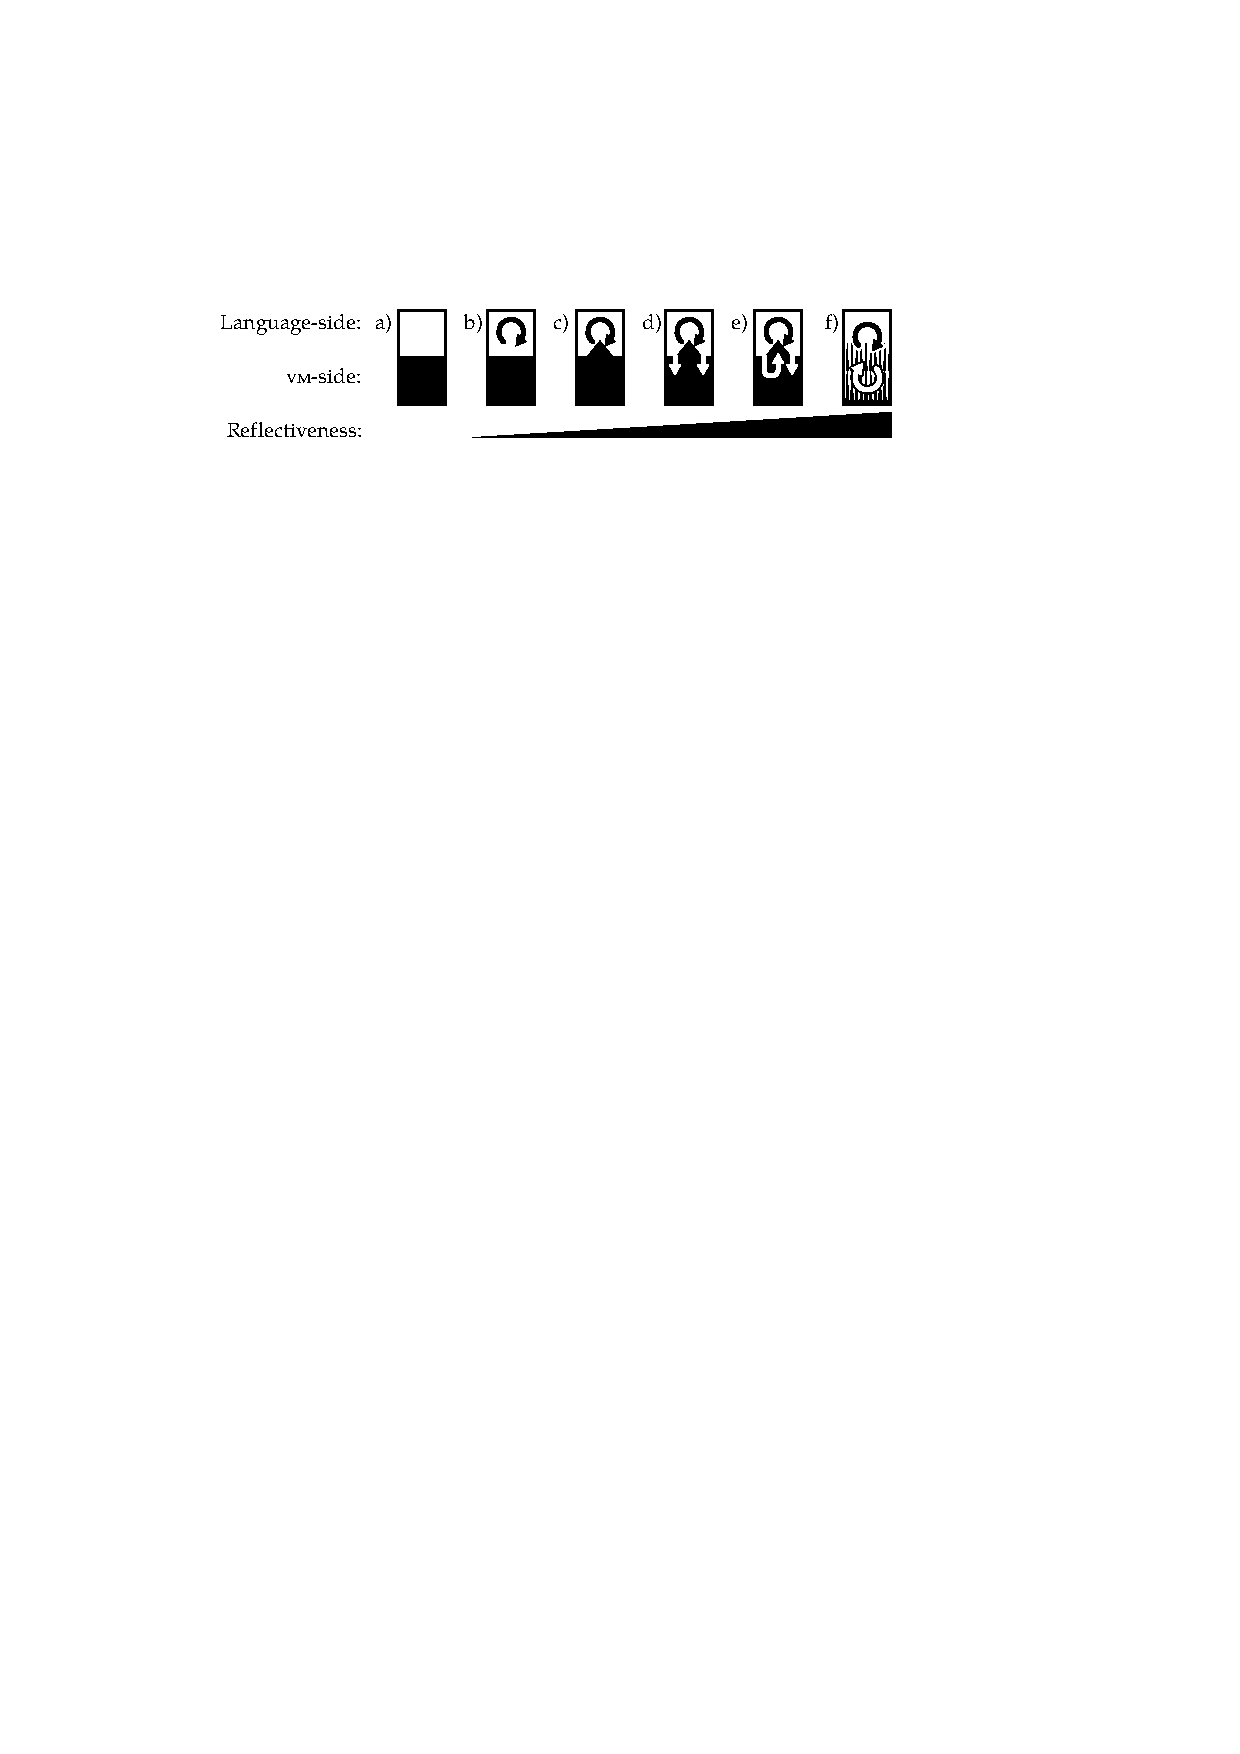
\includegraphics[scale=1.1]{vm-reflection-evolution}
\figlabel{vm-reflection-evolution}
\end{figure}

\begin{description}
\item[Language-side access to the \VM:]
\item[Language-side modification of the \VM:]
\item[Self-aware \VM:]
\end{description}

\todo{VM Generation Frameworks change the picture partially: full reflection at compile-time}\\
\todo{The 4th Quadrant! same reflection capabilities of vm framworks at runtime}

\todo{Mini example / introduction: \JIT}\\
\begin{stcode}{}
VM gc addGCSpace: MyCustomGCSpace new.
\end{stcode}


% ===========================================================================
\section{Open \VMs}
\seclabel{background-open-vms}
% ===========================================================================
\todo{Simple History of \VMs: static frames, high abstraction mismatch}\\
\todo{missign structural refleciton => go towards \VM frameworks} \\
\todo{At the same time hard requirements which can only be achieved with very low-level programming}\\

% ---------------------------------------------------------------------------
\subsection{Metacircular \VMs}
\seclabel{background-metacircular-vms}
% ---------------------------------------------------------------------------
\todo{Ultimate Goal: Run the \VM in the same language... what do we improve by that?}\\
\todo{  lesser abstraction mismatch, known tools, better debugging, faster development }\\
\todo{Image different approaches 2 axis: lanugage properties(absorbed / explicit), bootstrap (intermediate, direct)}

\paragraph{Language Property Synthesis}
\todo{Where does the implemented lanugage properties come from: managed vs. explicit}.
\todo{Eraly approaches like the \Squeak \VM have no absorption}\\
\todo{Typical \VM generation framweork, akak. facny C or C++ (mimics their final staticness while being more flexible during pre-compilation)}\\
\todo{\PyPy gives not direct access to the underlying \JIT implementation, plug and play}\\
\todo{Very high-level interface}\\
\todo{Truffle as extreme to that track: Interpreter implementation on \AST basis, not explicit bytecode interpreter (which would be typical in C)}

\paragraph{Bootstrap Process}
\todo{Early approaches use C as intermeditate representation}\\
\todo{Implies the whole GCC stack} \\
\todo{Hard to circumvent GCC's limitations => generate own native code} \\
\todo{Fluent transition from purely C based bootstrap, over C-kernel + native code to purely native code} 


% ---------------------------------------------------------------------------
\subsection{Compile-time Reified \VMs}
% ---------------------------------------------------------------------------

\subsubsection*{\Squeak \ST \VM}
\seclabel{background-squeak}
% ---------------------------------------------------------------------------
\todo{Does not absorb any properties} \\
\todo{\ST used as C template engine}

\WF is implemented in \PH which uses the \urlfootnote{\Cog \VM}{http://www.mirandabanda.org/cogblog/}, originating from the \Squeak \VM\cite{Inga97a}.
The \VM itself is written in a dialect of \ST called \Slang that is essentially limited to the functionality that can be expressed with standard C code.
\Slang serves for two purposes: a high-level C preprocessor, a interactive simulator of the \VM.
The first point has severe consequences.
\Slang basically has the same syntax as \ST but is semantically constrained to expressions that can be resolved statically at compilation or code generation time and are compatible with C.
Hence \Slang's semantics are closer to C than to \ST.
This fact is also visible in the simulator for the \VM.
If \Slang were \ST, separate parts of the \VM could be directly evaluated.
However, since \Slang is bound to C expressions, the simulator sets up a byte array as memory.
The simulated \VM then accesses this byte array as if it were the native memory.

In conclusion we see that the \PH \VM has an abstract representation of the \VM available for simulation.
This abstract representation is then used to generate C sources, already lowering the abstraction level.
After compiling the C sources the original representation of the \VM is not directly accessible anymore.
For instance, even debug symbols are usually stripped from the final binary for performance reasons.
Of course this implies that the \VM can not be changed nor directly inspected from language-side.


% ---------------------------------------------------------------------------
\subsubsection*{High-level low-level Programming in \Jikes with \MMTK}
\seclabel{background-jikes}
% ---------------------------------------------------------------------------
\todo{Image: Infrastructure Overview}

High-level low-level programming \cite{Fram09a} advocates using high-level languages for system programming.
Frampton et al. present a low-level framework packaged as \ttt{org.vmmagic}, which is used as system interface for Jikes, an experimental Java VM.
Additionally their framework is successfully used in a separate project, the memory management toolkit (\MMTK) \cite{Blac04a} which is used independently in several other projects.
The \ttt{org.vmmagic} package introduces highly controlled low-level interaction in a statically type context.
Methods have to be annotated to use low-level functionality. 

The \ttt{org.vmmagic} package is much more elaborate than \NB, notably their type system extensions allow for optimized interaction between several low-level methods.
\cb{do we need to list more what they do?}
However as we state in the introduction, it is tailored towards Java with static types.
Additionally the strong separation between low-level code and runtime does not allow for reflective extensions of the runtime.

% ---------------------------------------------------------------------------
\subsubsection*{\Maxine \Java \VM}
\seclabel{background-maxine}
% ---------------------------------------------------------------------------
\Maxine is a metacircular \Java \VM \cite{Wimm13a} focused on an efficient developer experience.
The \Maxine \VM stands out as it truly focuses on productivity and developer interaction.
\Maxine uses abstract and high-level representations of \VM-level concepts and consistently exposes them throughout the development process.
Inspectors at multiple abstraction levels are readily available while debugging, giving insights to the complete \VM state.
\Maxine provides and excellent navigation for generated native code by providing links back to language-side objects as well as other native code and symbols.

Compared to \Maxine, the \B infrastructure currently lacks the debugging tools which would enable a truly seamless interaction with the low-level world.
Namely, \B does not support low-level debugging and does not support facilities to inspect low-level native code directly.
However, \Maxine focuses on \Java, a language with inferior reflective capabilities compared to \PH.
Hence the live interaction with the \VM is only possible during the development phase and not exposed to the language-side.


\subsubsection*{\PyPy}
\seclabel{background-pypy}
% ---------------------------------------------------------------------------
\urlfootnote{\PyPy}{http://pypy.org/} is a \Python-based high-level \VM framework \cite{Rigo06a}.
\PyPy's major focus lies on an efficient metacircular \Python interpreter.
However, it has been successfully used to build \VMs for other languages including \ST \cite{Bolz08a}.
Interpreters are written in a type-inferable subset of \Python called \RPython.
The underlying \PyPy infrastructure implicitly provides memory management and \JIT compilation.

\paragraph{Provided \VM Features}
\PyPy follows a different approach from the previously presented \VM generation frameworks.
For instance, in Squeak and \Jikes the final \VM implementation is not much different from C or C++.
The programmer specifies all the components of the \VM explicitly, either by implementing them directly or using a provided library.
Compared to the more static C ans C++ these \VM generation frameworks make the compilation phase more tangible.
\ST in \Squeak or \Java in \Jikes or \Maxine fulfill the purpose of the template system in C++ or the restricted macro system in C.
For the explicit implementation part \PyPy is no different.
However, certain features for the final \VM are directly absorbed from the underlying \PyPy infrastructure.
For instance, the \JIT support or the \GC are not explicitly implemented but provided by the \PyPy framework itself.
This is a big difference to the other \VM frameworks as it allows programmers to write the \VM in a more high-level fashion.
For instance in \Squeak memory allocation, even for \VM-level objects, has to be handled in the same way as in C.
Whereas in \PyPy the garbage collection is left to the underlying infrastructure.

\paragraph{\RPython Interpretation}
At compile-time the interpretation stack for a newly implemented \VM on top of \PyPy looks as follows.
%
\begin{enumerate}
\item The final language runtime
\item The \VM written in \RPython
\item The \PyPy infrastructure (virtual compile-time \RPython interpreter)
\end{enumerate}
%
Unless in debug mode, the bottom-most layer is compiled away by exporting the \RPython sources to C.
However, before the C export step, all the compile-time reflection statements are evaluated and flattened away.
This approach allows \RPython \VMs to behave almost like standard \Python programs while still providing excellent performance in the final \VM binary.

\paragraph{High-level Tracing \JIT}
Much like the automatic memory management, \PyPy provides a tracing \JIT generator \cite{Bolz09a}.
By default the \VM programmer does not write an explicit \JIT in \PyPy.
Instead the \VM code is annotated to guide the underlying tracing \JIT generator.
This means a \VM compilation time a specific tracing \JIT is created for the given meta information.
As a result, the \JIT can track high-level loops in the final interpreted language.

\todo{in that sense maybe also add truffle}


% ---------------------------------------------------------------------------
\subsection{Runtime Reified \VMs}
\seclabel{background-reified-vms}
% ---------------------------------------------------------------------------

The \VMs presented so far have little or no self-awareness.
Typically the \VM generation frameworks only allow a high amount of reflection at \VM compile time.
This meta information is typically compiled away, similar to a C++-based \VM.
The \VM frameworks themselves behave like a static language on their own.
The final \VM artifact has no access to the underlying definition anymore.
Typically some structural meta information is available at runtime but not made available to the language running on top.

We are now going to present \VMs that behave significantly different.
These \VMs have direct control over the underlying infrastructure and most concepts
\cb{yadda yadda yadda}
\todo{need proper link from static VM to dynamic VM}\\
\todo{draw parallel to C (classical VM), vs C++ (Maxine / Jikes), Java (PyPy) vs someting like ST} \\
\todo{probably add table for comparison}\\
\todo{Proper separation \cite{Wimm12a} at compile time should make it easy to push it to dynamic/runtime}


% ------------------------------------------------------------------------------
\subsubsection*{\Pinocchio \VM}
\seclabel{background-pinocchio}

The \P \VM \cite{Verw11a} presented in \secref{background-pinocchio} is a direct predecessor of the work presented in this thesis.
The knowledge gained while participating on \P had a great influence on the development direction of \B and its applications.

Unlike \PH running on the \Cog \VM the \P research \VM has no bytecode interpreter.
The only execution base is native code which is directly generated by the language-side compiler.
At the current stage of development \P has not yet support for a separate image as in \PH.
The runtime image is currently defined by the bootstrap process where classes, objects and methods are exported into binary images and linked together with a primitive kernel to a final executable.

\paragraph{Going Native}
We took from \P that language-side native code generation is not more complex than generating bytecodes.
Instead we directly embrace the native world.
This means that in the core \P already uses many concepts that are only introduced by the \JIT in the \Cog \VM.
Hence, \P does no longer distinct between \JIT mode and interpreter mode.
Here the gain for \P are twofold: we could boost the performance of the language-runtime and simplify the design by not needing a dual compilation pipeline for the \JIT and the bytecode.

\paragraph{Going Meta}
Even so \P directly uses native code as core execution mode we avoided to directly write native code if possible.
For instance the method lookup in \Cog is statically implemented at \VM-side using \Slang.
We described in \secref{background-pinocchio} in detail how \P uses language-side code instead for the lookup.
Using the combination of low-level code to flatten out meta recursion we still have full language-side control over the lookup while maintaining good performance.

\paragraph{Missing Low-level Reification}
The most obvious shortcoming of \P was the lack of its own garbage collector.
Instead of investing time into a separate well-defined \GC \P relies on the conservative \urlfootnote{Boehm \GC}{http://www.hpl.hp.com/personal/Hans_Boehm/gc/} built for C programs.
The Boehm \GC is sufficiently fast to run \P as a prototype, however, due to its generic nature it is not as efficient as a specific \GC.
However, \P lacked the necessary reification at level of the object layout to properly implement a \GC.
All the notion about the object layout in memory are hard-coded in the compiler in several places.

\todo{no real distinction between \JIT and interpreter} \\
\todo{compiler directly generates native code} \\
\todo{simplified infrastructure} \\
\todo{lagnuage-side: lookup links back to language-side code with prefilled native code to avoid meta recursion}
\todo{missing reification for the layout (work in progress)} \\
\todo{missing reification for low-level \VM objects} \\
\todo{still used minimal C kernel for simplicity} \\
\todo{required gcc + linker for bootstrap}

% ------------------------------------------------------------------------------
\subsubsection*{\MIST a C-less \ST Implementation}
\urlfootnote{\MIST}{http://mist-project.org/} is another prototype \ST \VM that follows similar goals as the \P \VM.
It not longer uses bytecode interpreter but only relies on native code.
However, it goes one step further than \P by not relying on any C-based infrastructure.
\MIST implements its own linker to build the final executable.
And unlike \P it does not require kernel primitives written in C.
\MIST brings its own implementation to directly perform system calls from within the language.

% ------------------------------------------------------------------------------
\subsubsection*{\DwarfPython}

\todo{see \cite{Kell11a}}
\todo{History based on \Parathon + \Dwarf}\\
\todo{explain unified \VM runtime model}\\
\todo{language-runtime controls everything}\\
\todo{user for better low-level interaction}\\
\todo{shared infrastructure for \FFI callout generation}\\

% ------------------------------------------------------------------------------
\subsubsection*{\Klein \VM}
\seclabel{background-klein}
\urlfootnote{\Klein}{http://kleinvm.sourceforge.net/} is a metacircular \VM for the \Self programming language that has no separation into \VM and language \cite{Unga05a}.
The \VM is entirely written in \Self but takes the concept of metacircular beyond the compile-time.
For instance, unlike many other metacircular \VMs, including \Cog and \Squeak, \Klein does not use an intermediate low-level language to bootstrap the system.
It generates directly a binary image, much like the aforementioned \P or \MIST \VM.
However, it is important to note that the \VM-level structures and objects are not compiled away as it is usually the case.
Instead the \VM structures are represented as real \Self objects.
Hence the \Klein \VM supports true \VM-level reflection since there is only a single code base.

Additionally to the advances in reflection and metacircularity, \Klein focuses on fast compilation turnarounds to allow for a responsive development process.
Which is unlike the \Squeak \VM where a full \VM bootstrap takes a order of minutes on modern hardware.
\Klein also supports advanced mirror-based debugging tools to inspect and modify a remote \VM.

Development on the \Klein \VM seized in 2009 and left the \Klein \VM in fairly usable state.
However, up to now it lacks a proper \GC which essentially limits its real-world application.
Yet, it proved that it is possible and build a language-runtime without a proper separation of the language-side and the \VM or base-level.
From the literature presented about the \Klein project we see a strong focus on the improvements of the development tools.
The fact that the language-runtime allows \VM-level reflection to change the \VM dynamically is not directly mentioned in the literature.
While we see the practical limitations of changing the \VM at runtime we would like to open the doors to this new form of reflection.
\todo{reread paper}
\todo{Image: Infrastructure Overview}


\section{Tools Accessing the VM}
\todo{properly integrate into the rest}

\subsection*{\Quicktalk}
\Quicktalk \cite{Ball86a} follows a similar path as we do with Waterfall presented in \secref{waterfall}.
However Ballard et al. focus mostly on the performance aspect.
They achieve higher performance mostly by eliminating the bytecode dispatch overhead.
Additionally they type annotate the code for the primitive definitions to benefit from further optimizations.
\WF however, is a very lightweight approach that provides less optimization opportunities on a general code base.
\Quicktalk tries to compile generic \ST code, where Waterfall is mainly applied to single limited primitives.


\subsection*{\DTrace}
\cb{maybe remove the dtrace discussion from here and move it into the waterfall section and cite \cite{Cant04a} there}
\todo{see \cite{Cant04a}}


% ===========================================================================
\section{Problem 1: }
% ===========================================================================


% ===========================================================================
\section{Problem 2: }
% ===========================================================================


% ===========================================================================
\section{Problem 3: }
% ===========================================================================


% ===========================================================================
\section{Summary and Outlook}
% ===========================================================================

\todo{Intro + List again the problems} \\
\todo{Sync Chapter Outlook}


% =============================================================================
\ifx\wholebook\relax\else
    \end{document}
\fi